\subsection{Fundamentals of Survival Analysis} \label{Fundamentals of Survival Analysis}

In survival analysis, the random variable $Y$ represents the time until an event of interest occurs (e.g., death or failure). The distribution of $Y$ is commonly described by the following fundamental functions (\cite{kleinbaum1996survival}):
\begin{enumerate}
    \item \textbf{Survival function}, which gives the probability that the event has not occurred by time $y$:
   $$
   S(y) = P(Y > y) = 1 - F(y).
   $$
   \item \textbf{Probability density function (PDF)}, which represents the instantaneous probability density of the event occurring exactly at time $y$:
   $$
   f(y) = \frac{d}{dy} F(y).
   $$
   \item \textbf{Hazard function}, defined as:
   $$
   h(y) = \lim_{\Delta y \to 0} 
   \frac{P(y \le Y < y + \Delta y \mid Y \ge y)}{\Delta y}
   = \frac{f(y)}{S(y)},
   $$
   It represents the instantaneous risk that an event occurs within an infinitesimally small time interval, given that the individual has survived up to time \( y \).
\end{enumerate}

The relationships among these functions are:
$$
f(y) = h(y) S(y),
\quad
S(y) = \exp\Big( - \int_0^y h(u) du \Big).
$$
Therefore, these three functions can be derived from each other and jointly describe the probabilistic behavior of the survival time.


\subsection{Why Bayesian}\label{Why Bayesian}
When we first encounter survival analysis, it may seem sufficient to estimate the risk rate $\lambda$ with a single best value (for example, via Maximum Likelihood Estimation, MLE). However, as we begin to truly reflect on the relationship between data and models, we realize that merely obtaining a point estimate is far from enough. For instance, under the exponential survival model, we maximize the likelihood function (\cite{ibrahim2013bayesian}):
$$
L(\lambda) = \prod_{i=1}^{n} [\lambda e^{-\lambda y_i}]^{\delta_i} [e^{-\lambda y_i}]^{1 - \delta_i}
$$
This formula tells us how to find the most likely value of $\lambda$, but it does not tell us: how uncertain is this estimate? In real-world applications, we often need more than a single number. We want to understand the plausible range of this value given the data. This is precisely where the Bayesian approach fills the gap. The core of Bayesian inference is that it treats parameters not as fixed unknowns but as random variables (\cite{bartovs2022informed}). Through the formula:
$$
\text{Posterior}(\lambda \mid data) \propto \text{Likelihood}(data \mid \lambda) \times \text{Prior}(\lambda)
$$
It combines prior knowledge (Prior) with the information provided by the current data (Likelihood), yielding the posterior distribution (Posterior). This inference framework shows that the integration of data and prior knowledge is not an either-or choice, but a continuous process of updating and refinement.

In the context of survival analysis, the advantages of Bayesian methods become even clearer (\cite{bartovs2022informed}). Firstly, survival data are typically censored. In the Bayesian framework, censored observations are naturally incorporated into the likelihood—the likelihood contribution of a censored sample is simply its survival function $S(y) = e^{-\lambda y}$. Secondly, Bayesian methods allow us to incorporate historical information or expert opinion as priors. This is particularly useful when the sample size is small or the censoring proportion is high, providing more stable parameter estimates. Thirdly, the Bayesian framework is inherently extendable. From the simple exponential model to more complex Weibull models, or even to non-parametric and semi-parametric models, we only need to adjust the definitions of the likelihood and prior to obtain structured posterior inference, ensuring model interpretability and stability.

Thus, adopting a Bayesian approach is not merely a technical choice, but an expression of a more honest and deeper understanding of uncertainty. In survival analysis, estimating parameters is not the hard part; the real challenge lies in fully capturing and communicating the uncertainty around those estimates, so that robust decisions can be made in practice. This is the fundamental advantage of Bayesian methods in survival analysis.











\subsection{Parametric Exponential Model} \label{Exponential Model}

The exponential model is one of the simplest and most classic Bayesian survival models, assuming a constant hazard rate over time:
$$
h(y) = \lambda.
$$
This implies that the instantaneous event risk remains unchanged regardless of survival time. For example, if a light bulb has the same failure risk at any moment, we only need to know $\lambda$ without modeling time-varying risks, simplifying inference and calculation.

In general, for any parametric survival model with density $f(y|\theta)$ and survival function $S(y|\theta)$ (\cite{enwiki:1270064454}), the likelihood is:
$$
L(\theta | D)
= \prod_{i=1}^n
[ f(y_i | \theta) ]^{\nu_i}
[ S(y_i | \theta) ]^{1 - \nu_i},
$$
where $\nu_i=1$ indicates an observed event (contributing $f(y_i|\theta)$) and $\nu_i=0$ indicates right-censoring (contributing $S(y_i|\theta)$). Thus, the likelihood combines exact failure information and partial censoring information coherently within a Bayesian framework.

For the exponential model (\cite{ibrahim2013bayesian}):
$$
S(y) = 
\begin{cases}
\exp\Big( -\int_0^y h(u) du \Big)=\exp(-\lambda y), & y \ge 0 \\
1, & y < 0 
\end{cases}
$$
$$
f(y) = 
\begin{cases}
h(y) S(y)=\lambda \exp(-\lambda y), & y \ge 0 \\
0, & y < 0
\end{cases}
$$
Including covariates via a log-link yields  (\cite{ibrahim2013bayesian}):
$$
\lambda_i = \exp(\mathbf{x}_i^\top \boldsymbol{\beta}),
\quad i = 1, \ldots, n,
$$
Without covariates, the hazard reduces to (\cite{chen2025survival}):
$$
\lambda_i = \exp(\beta_0),
$$
representing a single baseline hazard rate for all individuals. With covariates, $\lambda_i$ varies with individual characteristics.

Here $\boldsymbol{\beta}$ are regression coefficients, and the likelihood becomes:
\begin{align*}
L(\boldsymbol{\beta} | D)
&= \prod_{i=1}^n 
\big[ f(y_i | \boldsymbol{\beta}) \big]^{\nu_i}
\big[ S(y_i | \boldsymbol{\beta}) \big]^{1 - \nu_i} \\
&= \prod_{i=1}^n 
\big[ \lambda_i \exp(-\lambda_i y_i) \big]^{\nu_i}
\big[ \exp(-\lambda_i y_i) \big]^{1 - \nu_i} \\
&= \prod_{i=1}^n 
\lambda_i^{\nu_i} 
\exp(-\lambda_i y_i) \\
&= \prod_{i=1}^n 
\exp\big( \nu_i \mathbf{x}_i^\top \boldsymbol{\beta} \big)
\exp\big( - y_i \exp(\mathbf{x}_i^\top \boldsymbol{\beta}) \big).
\end{align*}
In Bayesian inference, we assign priors $\pi(\theta)$, either weakly informative (e.g. $\pi(\theta)\propto1$) or informative (e.g. $\boldsymbol{\beta} \sim N(\boldsymbol{\mu}_0, \Sigma_0)$). Priors stabilize estimation, especially with small samples.

Overall, Bayesian inference proceeds by specifying the model and prior, computing the posterior:
$$
\pi(\theta | D)
\propto
L(\theta | D) \times \pi(\theta),
$$
then summarizing it via means, medians, credible intervals, or posterior predictive distributions.

For example, with a normal prior, the (unnormalized) posterior is:
$$
\pi(\boldsymbol{\beta} | D)
\propto
L(\boldsymbol{\beta} | D)
\times
\pi(\boldsymbol{\beta}).
$$
With log posterior:
$$
\log \pi(\boldsymbol{\beta} | D)
\propto \sum_{i=1}^n
\big[ \nu_i \mathbf{x}_i^\top \boldsymbol{\beta}
- y_i \exp(\mathbf{x}_i^\top \boldsymbol{\beta}) \big]
- \frac{1}{2}
(\boldsymbol{\beta} - \boldsymbol{\mu}_0)^\top
\Sigma_0^{-1}
(\boldsymbol{\beta} - \boldsymbol{\mu}_0).
$$
As this posterior lacks a closed form, MCMC methods are used for sampling (\cite{stats5010006}). Here, we implement it via \texttt{brms} in R.

For instance, fitting the exponential model without covariates to the veteran dataset yields the posterior distribution of $\lambda$ (Figure ~\ref{fig:exp veteran}).

\begin{figure}[H]
    \centering
    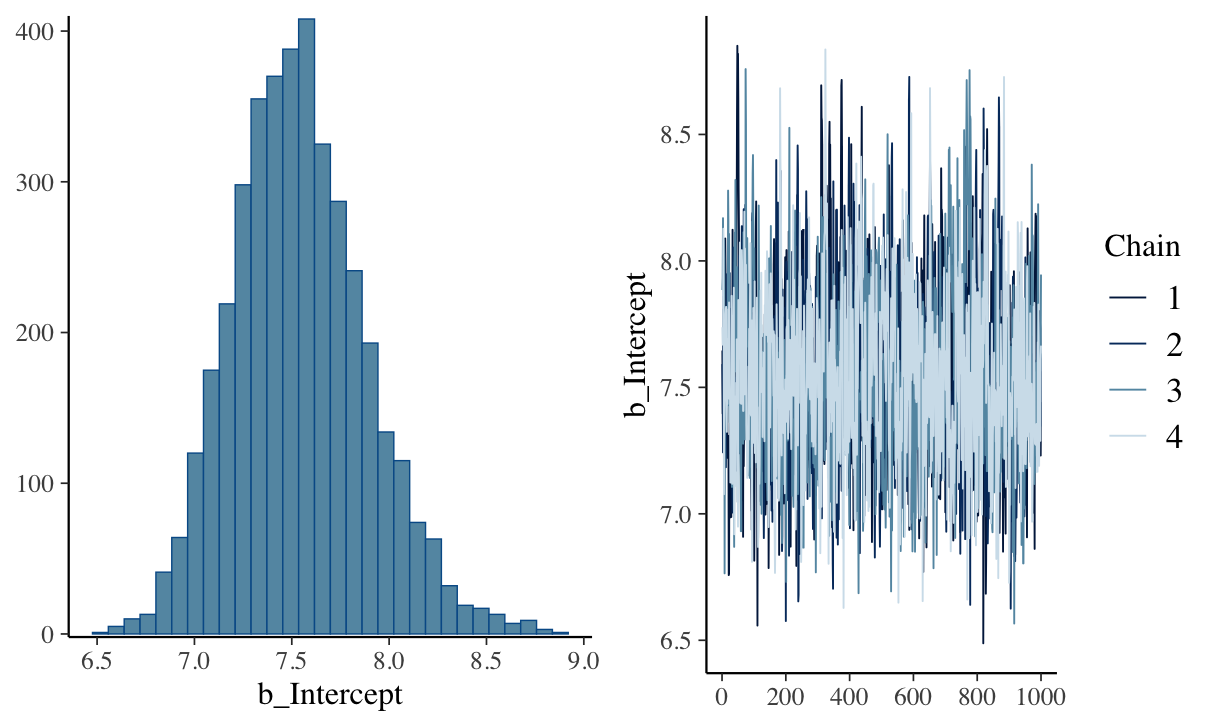
\includegraphics[height=6cm, width=0.9\textwidth]{MSc_Statistics_Research_Report_paper/images/exp model veteran.png}
    \caption{An example posterior density (left) and trace plot (right).}
    \label{fig:exp veteran}
\end{figure}
Posterior density plot shows the distribution and uncertainty of $\lambda$; Trace plot shows four MCMC chains with good mixing and convergence.





%%%%%%%%%%%%%%%%%%%%%%%%%%%%
%%%%%%%%%%%%%%%%%%%%%%%%%%%%%%
%%%%%%%%%%%%%%%%%%%%%%%%%



\subsubsection{Weibull Model} \label{Weibull Model}
The Weibull model is a natural generalization of the exponential model and is suitable for describing scenarios where the hazard rate changes monotonically over time. Compared to the exponential model, which assumes a constant hazard rate, the Weibull model introduces a shape parameter $\alpha$, allowing the hazard rate $h(y)$ to increase or decrease with survival time $y$, providing greater flexibility to capture realistic survival or failure patterns.

The hazard function, probability density function, and survival function are given by:
$$
h(y) = \alpha \gamma y^{\alpha - 1}, 
\quad 
f(y) = \alpha \gamma y^{\alpha - 1} \exp(-\gamma y^{\alpha}), 
\quad 
S(y) = \exp(-\gamma y^{\alpha}),
\quad \gamma > 0,
$$
where $\alpha$ is the shape parameter and $\gamma = \exp(\lambda)$ is the scale parameter. When $\alpha > 1$, the hazard rate increases over time (indicating an aging effect); when $\alpha < 1$, the hazard rate decreases over time (indicating early failure); and when $\alpha = 1$, the Weibull model reduces to the exponential model.

Similar to the exponential case, suppose the survival time sample $Y = (Y_1, \ldots, Y_n)$ is independently and identically distributed according to a common Weibull distribution. To further incorporate individual covariate effects, the scale parameter can be modeled as:
$$
\gamma_i = \exp(\mathbf{x}_i^\top \boldsymbol{\beta}),
\quad i = 1, \ldots, n,
$$
where $\mathbf{x}_i$ denotes the covariate vector and $\boldsymbol{\beta}$ is the vector of regression coefficients. The functional forms of the hazard and density remain unchanged, with $\gamma$ replaced by $\gamma_i$.
Assuming independent samples and right-censoring, the full likelihood function is:
$$
L(\boldsymbol{\beta}, \alpha)
= \prod_{i=1}^n 
\big[ f(y_i) \big]^{\nu_i} 
\big[ S(y_i) \big]^{1 - \nu_i}
= \prod_{i=1}^n 
\big[ \alpha \gamma_i y_i^{\alpha - 1} \big]^{\nu_i} 
\exp(-\gamma_i y_i^\alpha).
$$
For the prior specification, $\boldsymbol{\beta}$ can be assigned the same normal prior as in the exponential regression case, while the shape parameter $\alpha$ is commonly assigned a Gamma prior:
$$
\boldsymbol{\beta} \sim N(\boldsymbol{\mu}_0, \Sigma_0), 
\quad 
\alpha \sim \text{Gamma}(a_0, b_0).
$$
Assuming $\boldsymbol{\beta}$ and $\alpha$ are conditionally independent a priori, the joint posterior distribution (up to a normalizing constant) is:
$$
\pi(\boldsymbol{\beta}, \alpha | D)
\propto L(\boldsymbol{\beta}, \alpha)
\, \pi(\boldsymbol{\beta})
\, \pi(\alpha).
$$
Taking logarithms yields the log-posterior kernel:
$$
\log \pi(\boldsymbol{\beta}, \alpha | D)
= \sum_{i=1}^n 
\big[
\nu_i \log \alpha + \nu_i \mathbf{x}_i^\top \boldsymbol{\beta} 
+ \nu_i (\alpha - 1) \log y_i 
- \exp(\mathbf{x}_i^\top \boldsymbol{\beta}) y_i^\alpha
\big]
+ \log \pi(\boldsymbol{\beta}) + \log \pi(\alpha) + \text{const}.
$$
As in the exponential regression case, this posterior distribution does not have a closed form and must be sampled numerically. It can be shown that, given the normal prior for $\boldsymbol{\beta}$ and Gamma prior for $\alpha$, the log-posterior is concave with respect to each parameter, satisfying the log-concavity condition and making ARS or Gibbs sampling applicable for efficient inference.

\subsubsection{Extreme Value Model}
The Extreme Value (EV) model can be viewed as a reparameterization of the Weibull model in the log-time domain, which reformulates the hazard function as an exponential-linear form in log time, facilitating direct integration of covariates.

Specifically, if the survival time $T \sim \text{Weibull}(\alpha, \gamma)$, define:
$$
Y = \log T.
$$
Then,
$$
P(Y \le y) 
= P(\log T \le y)
= P(T \le e^y)
= F_T(e^y)
= 1 - \exp\big( - \gamma e^{\alpha y} \big).
$$
Therefore, the cumulative distribution function (CDF) for the EV model is:
$$
F(y) = 1 - \exp\big( - \exp(\lambda + \alpha y) \big), 
\quad \text{where}~\lambda = \log \gamma.
$$
It follows that:
$$
\begin{aligned}
S(y) &= \exp\big( - \exp(\lambda + \alpha y) \big),\\
f(y) &= \alpha \exp(\lambda + \alpha y) \exp\big( - \exp(\lambda + \alpha y) \big),\\
h(y) &= \alpha \exp(\lambda + \alpha y).
\end{aligned}
$$
Compared to the power-form hazard in the Weibull model, the hazard in the EV model becomes exponential-linear with respect to log time and covariates, making the derivation simpler, the interpretation more straightforward, and the link with covariates naturally linear. In this formulation, $Y \in (-\infty, +\infty)$ is no longer constrained to be positive.

With covariates, the location parameter is specified as:
$$
\lambda_i = \mathbf{x}_i^\top \boldsymbol{\beta}, 
\quad i = 1, \ldots, n.
$$
Accordingly,
$$
f(y_i) = \alpha \exp(\alpha y_i + \lambda_i) \exp\big( -\exp(\alpha y_i + \lambda_i) \big), 
\quad
S(y_i) = \exp\big( -\exp(\alpha y_i + \lambda_i) \big).
$$
The observations $\{ Y_i, \nu_i \}_{i=1}^n$ are assumed to be independent and identically distributed (i.i.d.).

The likelihood function is then:
$$
L(\boldsymbol{\beta}, \alpha) 
= \prod_{i=1}^n 
\big[ f(y_i) \big]^{\nu_i} 
\big[ S(y_i) \big]^{1 - \nu_i}
= \prod_{i=1}^n 
\big[ \alpha \exp(\alpha y_i + \lambda_i) \big]^{\nu_i} 
\exp\big( -\exp(\alpha y_i + \lambda_i) \big).
$$
The prior distributions are the same as for the Weibull model:
$$
\boldsymbol{\beta} \sim N(\boldsymbol{\mu}_0, \Sigma_0), 
\quad 
\alpha \sim \text{Gamma}(a_0, b_0).
$$
The joint posterior (up to a normalizing constant) is:
$$
\pi(\boldsymbol{\beta}, \alpha | D) 
\propto L(\boldsymbol{\beta}, \alpha)
\, \pi(\boldsymbol{\beta}) 
\, \pi(\alpha).
$$
The log-kernel of the posterior is:
$$
\log \pi(\boldsymbol{\beta}, \alpha | D)
= \sum_{i=1}^n 
\big[
\nu_i \log \alpha + \nu_i \alpha y_i + \nu_i \lambda_i - \exp(\alpha y_i + \lambda_i)
\big]
+ \log \pi(\boldsymbol{\beta}) + \log \pi(\alpha) + \text{const}.
$$
It can be shown that the Hessian of this log-posterior with respect to both $\boldsymbol{\beta}$ and $\alpha$ is non-positive definite, implying log-concavity, which allows safe and efficient inference using ARS or Gibbs sampling in practice.
